\qrchapter{https://forgottenpillar.com/rsc/hr-fp-chapter8}{Konstruktivna Kritika}

Prva točka \emcap{Fundamentalnih Principa} odgovara na pitanja: tko je Bog, što je Njegova ličnost, i kako razumijemo Njegovu prisutnost?

\others{I. Da postoji \textbf{jedan Bog}, \textbf{osobno, duhovno }\textbf{\underline{biće}}, \textbf{stvoritelj svih stvari}, svemoguć, sveznajuć, i vječan; beskonačan u mudrosti, svetosti, pravednosti, dobroti, istini i milosti; nepromjenjiv, i \textbf{svugdje prisutan po svojem predstavniku, Svetome Duhu}. Ps. 139:7.}[FP1889 147.2; 1889][https://egwwritings.org/read?panels=p931.6]

Jedan Bog, Stvoritelj, identificiran je kao Otac, jer druga točka \emcap{Fundamentalnih Principa} navodi da je Isus Krist, Sin Vječnog Oca, onaj po kome je Bog sve stvorio\footnote{\href{https://egwwritings.org/?ref=en_FP1889.147.3&para=931.7}{FP1889 147.3; 1889}}. \emcap{Ličnost Boga} izražena je izrazom “\textit{osobno duhovno biće}”. Uskoro ćemo vidjeti da ovaj izraz označava da Otac ima materijalno tijelo, fizičku manifestaciju. Dakle, u svojoj ličnosti, prisutan je samo tamo gdje fizički boravi. Ali, Njegova prisutnost nije ograničena Njegovom ličnosti jer je \others{svugdje prisutan po svojem predstavniku, Svetome Duhu.} Tijekom naše povijesti, ovo razumijevanje i rasuđivanje o \emcap{ličnosti Boga}, kako je izraženo u prvoj točki \emcap{Fundamentalnih Principa}, primilo je konstruktivnu kritiku; pod “konstruktivnom kritikom” mislimo na kritiku koja je poduprta Biblijom.

Sada vam predstavljamo sljedeće citate, neku konstruktivnu kritiku, od istaknutog trinitarijanca u svijetu Adventista Sedmoga Dana. Zanimljivo je da je on priznao autoritet \emcap{Fundamentalnih Principa}, a istovremeno vjerovao u doktrinu o Trojstvu. Smatramo ovaj dokument veoma važnim elementom u promjeni naših vjerovanja od fundamentalnih principa do trenutnog adventističkog trinitarijanskog vjerovanja.

Ovom bratu postavljeno je pitanje, “\textit{Ne vjerujete li u osobnog, opipljivog Boga?}”:

\others{\textbf{Zasigurno. Beskonačno, božansko, osobno biće je osnova religije}. Obožavanje zahtijeva nekoga voljeti, pokoravati mu se, vjerovati mu. \textbf{Vjera u osobnog Boga je sama srž kršćanske religije}. Koncepcija Boga kao Sva-Energija, beskonačna Moć, sveprožimajuća Prisutnost, prevelika je za ljudski um; mora postojati nešto \textbf{opipljivije}, nešto \textbf{\underline{ograničenije}}, na čemu se usredotočuje um u bogoslužju. \textbf{Iz tog razloga je Krist došao k nama na sliku Božje }\textbf{\underline{ličnosti}}\textbf{, drugog Adama, da bi nam svojim životom ljubavi i samopožrtvovnosti pokazao karakter i }\textbf{\underline{ličnost Boga}}. Bogu možemo pristupiti samo kroz Krista.}

\othersnogap{‘On, koji je odsjaj slave njegove, i \textbf{savršena slika Njegove osobe}, te koji nosi sve stvari riječju sile svoje, pošto kroz sebe izvrši očišćenje grijeha naših, sjede zdesna Veličanstvu u visinama.’}

\othersnogap{‘On, koji je sjaj slave njegove, i otisak njegove suštine, te koji drži sve stvari riječju svoje moći.’}

\othersnogap{Apostol kaže: ‘A mi svi koji otkrivenim licem slavu Gospodnju kao u zrcalu gledamo, u isti se lik preobražavamo iz slave u slavu, kao od Gospodnjega Duha.’ 2 Kor. 3:18. Koliko je lijepa ta slika!... Gledajući \textbf{Krista} u njegovim čudima, njegovim iskušenjima, njegovom uzvišenju, u njegovom životu samoodricanja, njegovom ‘išao je zemljom čineći dobro’, možemo promatrati \textbf{ličnost Boga i moć Božju}. A kako je samo velika nada za nas u činjenici da \textbf{u Kristu nalazimo kvalitete koje nisu čovjeku čudne i strane}, nego srodne mentalne i moralne osobine; tako da možemo vidjeti i shvatiti stvarnu, a ne samo teološku, apstraktnu ili figurativnu istinu, u izjavi apostola: ‘Sada smo djeca Božja.’ 1 Ivanova 3:2.}

\othersnogap{\textbf{Činjenica da je Bog tako velik da ne možemo stvoriti jasnu mentalnu sliku o njegovom \underline{fizičkom izgledu} ne treba umanjivati u našim umovima stvarnost \underline{ličnosti Boga}, niti ova koncepcija proturječi onoj posebnoj manifestaciji Boga u nekom \underline{određenom obliku ili mjestu}}. \textbf{Doista, postoje Biblijski tekstovi koji prikazuju Boga u ovom \underline{određenom} obliku, i može se reći \underline{ograničenoj formi}, da sjedi na prijestolju na nebu, ili da prebiva u hramu u Jeruzalemu}, 1. Kraljevima 22:19; Ps. 11:4; Matej 21:12, 13.}

\othersnogap{Ljudski um je ograničen i ne može shvatiti beskonačnost. \textbf{Prirodno želimo stvoriti određenu, jasno definiranu koncepciju bića koje obožavamo}. \textbf{Biblija zadovoljava ovu ljudsku potrebu kao i sve ostale naše duhovne zahtjeve, a }\textbf{\underline{u četrdesetom poglavlju Izaije}}\textbf{ prorok se bavi pitanjem Božjeg osobnog izgleda na čudesan način}. ‘O Jeruzaleme, ti koji donosiš dobre vijesti, podigni svoj glas snagom; podigni ga, ne boj se; reci gradovima Judinim, \textbf{Evo vašeg Boga}! On će hraniti svoje stado kao pastir; skupit će jaganjce u svoje naručje i nositi ih u svom naručju.’}

\othersnogap{‘Tko je svojom pregršći izmjerio vode i nebesa premjerio \textbf{pedljem}? Tko li je mjerilom razmjerio prah zemaljski i utezima odmjerio planine, a tezuljom brjegove? \textbf{S kime ćete dakle usporedit Boga?} \textbf{I s kakvim ga likom prispodobiti?} Zar ne znate? Zar niste čuli? Nije li vam od iskona objavljeno? Niste li razumjeli od utemeljenja zemlje? \textbf{To je onaj koji stoluje nad krugom zemaljskim}, čiji su pak stanovnici poput skakavaca; \textbf{ko zastor je razastro nebesa i ko šator ih za stan razapeo.} \textbf{\underline{S kime ćete me dakle usporediti i tko mi je ravan? veli Sveti.}} Podignite uvis oči svoje i razvidite: tko je to stvorio? Onaj koji na broj izvodi vojsku njihovu, on ih sve zove po imenu. Zbog velike snage njegove i jakosti sile njegove, nijedno ne izosta. Zar ne znaš? Zar nisi čuo? Vječni Bog, GOSPOD, Stvoritelj krajeva zemaljskih, nije se umorio niti je iznemogao. Njegov je razbor nedokučiv. Umornomu snagu daje, a nejakima krjepkost uvećava. I momci se umore i smalakšu, i mladići sustaju sveudilj. Ali koji čekaju na GOSPODA, snaga im se obnavlja; podižu se na krilima kao orlovi; trče i ne malakšu, hode i ne umaraju se.’ Izaija 40:9,11,12,18,21,22,25,26,28-31.}

\othersnogap{\textbf{Ovdje je čudesan opis Boga. Spominju se njegov dlan, njegova ruka, njegove grudi}. On je opisan kako ‘sjedeći na krugu zemlje’, odmjeruje nebo pedljem, drži vode u udubini svog dlana; \textbf{\underline{tako da nema sumnje da je Bog definitivno, stvarno, osobno biće}}. \textbf{Samo apstraktno načelo, zakon, sila ne može imati dlan, ruku. \underline{Bog je osoba}, premda je prevelik za naše shvaćanje, kao što Job kaže}, ‘Bog je velik i ne poznajemo ga.’ Job 36:26...}

\othersnogap{\textbf{\underline{Ovo veliko biće} je prikazano kako sjedi na krugu zemlje}. Orbita zemlje je promjera gotovo dvjesto milijuna milja. \textbf{Biće tako veliko da zauzima sjedište takvih razmjera je sasvim \underline{izvan našeg shvaćanja u pogledu njegove forme}}. \textbf{Prorok to prepoznaje, te \underline{odvraća našu pažnju od nagađanja o točnoj veličini i obliku Boga} pokazujući nam apsurdnost pokušaja da se čak i mentalna slika stvori, \underline{ukazujući da je to vrlo blisko idolopoklonstvu}. Vidi stihove 18-21}. Zatim nam pokazuje gdje možemo pronaći pravu predodžbu o Bogu, ukazujući nam na stvari koje je stvorio: ‘Podignite oči svoje uvis i pogledajte tko je stvorio ove stvari.’ Ovo je također bila Pavlova zamisao: ‘Jer ono nevidljivo njegovo, već njegova vječna moć i \textbf{\underline{Božanstvo}}, jasno se vidi od stvaranja svijeta, jer se razumije iz djela stvorenih; tako da nemaju ispriku.’ Rimljanima 1:20.}

\othersnogap{\textbf{\underline{Rasprave o obliku Boga su krajnje besmislene}, i služe samo da umanje naše koncepcije o onome koji je iznad svih stvari, i stoga se ne mogu usporediti u obliku, veličini, slavi ili veličanstvu s bilo čim što je čovjek ikada vidio ili što je u njegovoj moći zamisliti}. U prisutnosti ovakvih pitanja, moramo samo priznati našu glupost i nesposobnost, i pokloniti glave s strahopoštovanjem \textbf{u prisutnosti Ličnosti, Inteligentnog Bića} čije postojanje cijela priroda nosi određeno i pozitivno svjedočanstvo, \textbf{ali koje je daleko izvan našeg shvaćanja \underline{kao što su granice prostora i vremena}}.}

Kao što je ranije spomenuto, ovaj brat priznaje \emcap{Fundamentalne Principe}, ali vjeruje u Trojstvo. Evo kratkog sažetka njegove konstruktivne kritike o \emcap{ličnosti Boga}: Bog je određeno, stvarno, osobno biće koje ima oblik – \others{\textbf{Doista, postoje Biblijski tekstovi koji prikazuju Boga u ovom \underline{određenom} obliku, i može se reći \underline{ograničenoj} formi, da sjedi na prijestolju na nebu}}. Razlog zašto to zagovara je radi toga što vjeruje da je potrebno za nas, ograničena ljudska bića, imati određeni objekt štovanja. Ali on proširuje ideju o “\textit{ograničenom}” Bogu svjedočanstvom iz Izaije 40. poglavlja, koje dokazuje da je Bog\others{\textbf{\underline{sasvim izvan našeg shvaćanja u pogledu njegove forme}}}. Svaka vrsta konceptualizacije Božjeg bića, u bilo kojem obliku, slična je idolopoklonstvu. \others{\textbf{\underline{Rasprave o obliku Boga su krajnje besmislene}}}. Prava realnost ličnosti beskonačnog Boga je izvan našeg razumijevanja. Božja realna ličnost je više od tajne za naša ograničena razmišljanja. To je zato što je Bog\others{\textbf{daleko izvan našeg shvaćanja \underline{kao što su granice prostora i vremena}}}. Za ovog brata, razumijevanje \emcap{ličnosti Boga} samo kao određenog bića je na jedan način istinito, ali na drugi način neispravno. Istina je da se Bog predstavio u \others{\textbf{\underline{nekom određenom obliku ili mjestu}}}, jer \others{mora postojati nešto \textbf{opipljivije}, više \textbf{\underline{ograničenije}}, na kojemu se usredotočuje um u bogoslužju}. Jednostavno razumijevanje Boga kao određenog i opipljivog bića je ograničavajuće za Boga. Sažetak njegove kritike je da bi trebali formirati naše koncepte o Bogu izvan \others{\textbf{granice prostora i vremena}}.

Molimo vas da iskreno razmotrite razloge vjere ovog brata. Razumijevanje njegovih argumenata je važno jer je imalo značajnu ulogu u povijesti Crkve Adventista Sedmoga Dana, kao odvažan korak odstupanja od Fundamentalnih Principa. Ovi argumenti nisu trivijalni; vrlo su uvjerljivi i potičemo vas na njihovo promišljanje. Možda se slažete s njima, ali dopustite nam da razotkrijemo zabludu. Ovi citati su iz knjige dr. Kellogga “\textit{Živi Hram}”\footnote{\href{https://archive.org/details/J.H.Kellogg.TheLivingTemple1903}{Dr. J. H. Kellogg, The Living Temple, str.29-33.}}. Iz odjeljka pod nazivom “\textit{Beskonačna Inteligencija kao Osobno Biće}”, stranice 29 do 33, odlomci izražavaju Kelloggov stav o \emcap{ličnosti Boga}, što je bio glavni problem s njegovom knjigom.

To što ste upravo pročitali je upravo ono na što je sestra White mislila kada je rekla: \egwinline{Imam nekoliko stvari za reći našim učiteljima \textbf{u svezi sa novom knjigom Živi Hram}. \textbf{Budite oprezni kako podupirete sentimente ove knjige \underline{glede ličnosti Boga}}. Kako mi je Gospod pokazao stvari, \textbf{ovi sentimenti ne nose odobrenje Božje}. \textbf{One su zamka koje je neprijatelj pripremio za ove posljednje dane}...}[Lt211-1903.1; 1903][https://egwwritings.org/read?panels=p14068.9598008]

U trenutnoj kontroverzi u adventističkoj crkvi u vezi s doktrinom o Trojstvu, osobno smo pokušavali preusmjeriti kontroverzu s doktrine o Trojstvu na \emcap{ličnost Boga}. Kada god bi smo predstavili stav prve točke \emcap{Fundamentalnih Principa}, naišli bi na protu argumente koji se u velikoj mjeri preklapaju s Dr. Kelloggovim vjerovanjem o \emcap{ličnosti Boga}, zagovaranom u “\textit{Živom Hramu}”. Ta situacija se uzastopno ponavlja. Kada se fokus pomakne s pitanja Trojstva na \emcap{ličnost Boga}, Kelloggovi pogledi o \emcap{ličnosti Boga} često odzvanjaju kod zagovornika doktrine o Trojstvu. Kvaliteta ili stanje koja Boga čine osobom je misterij u doktrini o Trojstvu, i često Kelloggovo vjerovanje o \emcap{ličnosti Boga} preklapa se s trinitarijskim razumijevanjem Božje ličnosti.

\begin{figure}[hp]
    \centering
    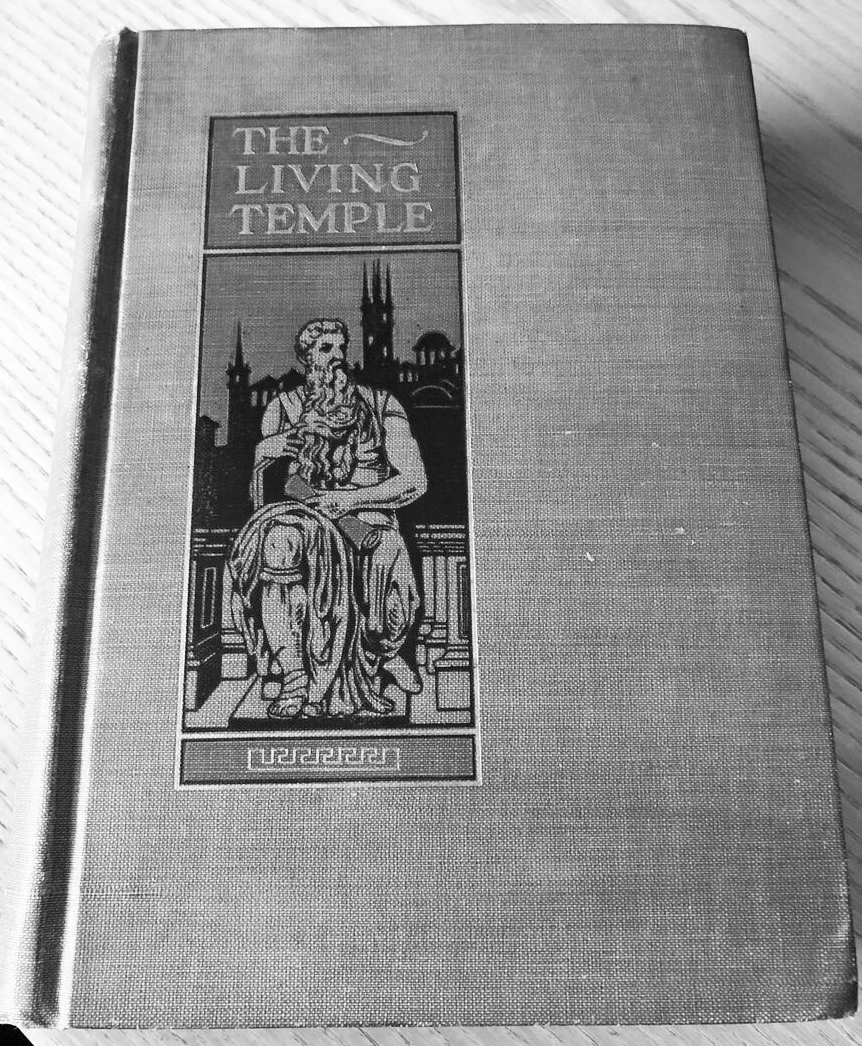
\includegraphics[width=1\linewidth]{images/TLT.jpg}
    \caption*{The Living Temple, Dr. J. H. Kellogg, 1903}
    \label{fig:tlt}
\end{figure}

Neki ljudi čije razumijevanje \emcap{ličnosti Boga} se preklapa sa razumijevanjem Dr. Kellogga, padaju pod iskušenje misliti da postoje neke druge sporne stvari u Živom Hramu, od ovih navedenih. Sljedeći pokazatelji sugeriraju upravo suprotno. Postoji pismo od Dr. Kellogga Williamu C. Whiteu, u kojem Dr. Kellogg predlaže \others{rezanje nekoliko stranica} iz tri tisuće primjeraka Živog Hrama—upravo onih stranica na kojima se pojavljuju \others{posebno sporne stvari, poput komentara na Izaiju 40} i vjerovanje o \emcap{ličnosti Boga} (upravo stranice koje smo čitali).

\others{Sanatorij ima na raspolaganju, otkrio sam, \textbf{dvije ili tri tisuće knjiga koje su prodane}, ali koje su vraćene otkako je knjiga osuđena. Postavilo se pitanje, što učiniti s njima? \textbf{Palo mi je na pamet da ih možda možemo spasiti \underline{rezanjem nekoliko stranica} na kojima se pojavljuju \underline{posebno sporne stvari}, poput \underline{komentara na Izaiju 40}, koji sam posudio od A.T. Jonesa, i stranice na kojoj se pojavljuje nesretni naslov ‘\underline{Ličnost Boga},’ i umetanjem stranica koje sadrže jasnu izjavu biblijskog pogleda na Boga kao osobe prezentiranu u članku starješine Haskella u ‘Reviewu’ prije nekoliko tjedana}. Ove knjige bi se prodavale starim pacijentima koji jako traže knjigu za božićne poklone...}[Pismo od Dr. J.H. Kellogga W.C.Whiteu; 6. prosinca 1903., Chicago][https://174625.selcdn.ru/ellenwhite/EWhite/17226/17226.pdf]

Koji je stvarni problem u rezoniranju o \emcap{ličnosti Boga} u Živom Hramu? Proučit ćemo to pitanje do same srži; no površno gledano, jasno vidimo da je problem odstupanje od temelja naše vjere—\emcap{Fundamentalnih Principa}—u pogledu \emcap{ličnosti Boga} i gdje je Njegova prisutnost.

\egw{\textbf{Bila sam upućena od strane Nebeskog glasnika} da su \textbf{neka rasuđivanja} u knjizi ‘Živi Hram’ netočna i da će \textbf{ta razmišljanja odvesti u zabludu} umove onih koji nisu temeljito utemeljeni na \textbf{temeljnim principima} sadašnje istine. \textbf{Ona uvode ono što je ništa više nego obična nagađanja} u \textbf{vezi ličnosti Boga i gdje je Njegova prisutnost}.}[SpTB02 51.3; 1904][https://egwwritings.org/read?panels=p417.262]

Dr. Kellogg je uveo razmišljanja \egwinline{koje su ništa više nego obična nagađanja vezano za ličnost Boga}, čime je odstupio od temelja naše vjere—\emcap{Fundamentalnih Principa}. Neslaganje između Kelloggovog učenja i \emcap{Fundamentalnih Principa} nalazi se u prvoj točki koja kaže da \others{postoji \textbf{jedan Bog}, \textbf{osobno, duhovno \underline{biće}}, \textbf{stvoritelj svih stvari}, ... i \textbf{svugdje prisutan po svojem predstavniku, Svetome Duhu}. Ps. 139:7.}

Sestra White nas je izravno upozorila na sentimente izražene u Živom Hramu u vezi s \emcap{ličnosti Boga}. Oni nisu u skladu s prvom točkom \emcap{Fundamentalnih Principa}, koji su bili dio temelja naše vjere.

\egw{\textbf{Morala sam mnogo pisati o čudnim doktrinama i teorijama izraženim u ‘Živom Hramu’. \underline{Ukoliko bi se ove teorije prihvatile od strane našeg naroda, jaki stupovi naše vjere i istine koje su učinile Adventiste Sedmog Dana onim što jesu, bile bi odstranjene}. Morala sam pokazati neispravnost ovih doktrina, predstavljajući ih \underline{kao vrstu hereze posljednjih dana}. Riječ Božja nam kaže da će upravo takvo učenje \underline{biti uvedeno u ovo vrijeme}.}}[Lt250-1903.2; 1903][https://egwwritings.org/read?panels=p9337.8]

Danas svjedočimo širokom prihvaćanju Kelloggovih teorija o \emcap{ličnosti Boga}. Činjenica da prva točka \emcap{Fundamentalnih Principa} više nije prisutna u našem vjerovanju, dokazuje da su Kelloggove teorije o \emcap{ličnosti Boga} imale utjecaj na oblikovanje naših vjerovanja.

\egw{Jedan za drugim dolaze k meni, tražeći me da \textbf{objasnim stajališta u knjizi ‘Živi Hram’.} Odgovaram, ‘Oni su neobjašnjivi.’ \textbf{Izraženi sentimenti ne daju istinsko znanje o Bogu. Kroz cijelu knjigu su odlomci Svetog Pisma}. \textbf{Pismo je korišteno na takav način \underline{da se zabludu prikaže kao istinu}}. \textbf{Pogrešne teorije su prikazane na tako ugodan način da, ukoliko se ne bude oprezan, mnogi će biti zavedeni}.}[SpTB02 52.1; 1904][https://egwwritings.org/read?panels=p417.265]

Zabluda se prikazuje kao istina, i mnogi su zavedeni.

Vrijedno je naglasiti, za neke nepažljive čitatelje, da pravi problem Dr. Kellogga i njegove knjige “\textit{Živi Hram}” nije Trojstvo nego mali korak koji je napravio odstupajući od \emcap{Fundamentalnih Principa}. Da bismo razumjeli pravi problem njegove knjige, bilo bi pogrešno fokusirati se na preklapanje njegovih sentimenata s doktrinom o Trojstvu. Umjesto toga, trebali bismo se fokusirati na točku koja je činila taj mali korak koji je napravio; a to uključuje duboko razumijevanje \emcap{fundamentalnih principa} baš kao što su ih naši pioniri imali. Koga boljeg pitati nego same adventističke pionire?

% Constructive Criticism

\begin{titledpoem}
    \stanza{
        Jedan Bog, osobno biće, Stvoritelj svih stvari, \\
        Po Duhu svugdje prisutan, tako nauk stari. \\
        Temelj vjere naše, princip fundamentalni, \\
        Istina što stoji čvrsto, stup naš kapitalni.
    }

    \stanza{
        Al' dođe kritika što zvuči mudro, fino, \\
        "Božja forma izvan shvaćanja," rekoše nevino. \\
        "Rasprave o obliku Boga besmislene su," \\
        Dok Kellogove riječi zamku postavljahu.
    }

    \stanza{
        "Bog je veći od prostora i vremena," tvrdiše, \\
        Dok od temelja vjere polako odstupiše. \\
        Pismo sveto koristiše da zabludu sakriju, \\
        Da ličnost Božju u misterij pretvore, žele liju.
    }

    \stanza{
        Jedan mali korak od principa učiniše, \\
        A stupove vjere naše time srušiše. \\
        Čuvajmo se teorija što zvuče uzvišeno, \\
        Jer u njima često leži zlo prikriveno.
    }

    \stanza{
        Bog je stvaran, određen i osoban zaista, \\
        To je istina što ostaje zauvijek čista. \\
        Ne dajmo da nagađanja zamijene nam znanje, \\
        Niti da nam misterij postane vjerovanje.
    }
\end{titledpoem}